	\documentclass[10pt,oneside]{CBFT_article}
	% Algunos paquetes
	\usepackage{amssymb}
	\usepackage{amsmath}
	\usepackage{graphicx}
	\usepackage{libertine}
	\usepackage[bold-style=TeX]{unicode-math}
	\usepackage{lipsum}

	\usepackage{natbib}
	\setcitestyle{square}

	\usepackage{polyglossia}
	\setdefaultlanguage{spanish}


	\usepackage{CBFT.estilo} % Cargo la hoja de estilo

	% Tipografías
	% \setromanfont[Mapping=tex-text]{Linux Libertine O}
	% \setsansfont[Mapping=tex-text]{DejaVu Sans}
	% \setmonofont[Mapping=tex-text]{DejaVu Sans Mono}

	%===================================================================
	%	DOCUMENTO PROPIAMENTE DICHO
	%===================================================================

\title{CBFT Mecánica clásica}
\author{Fuerzas centrales}
\date{\today}

\begin{document}
\maketitle
\tableofcontents

% =================================================================================================
\section{Fuerzas centrales}
% =================================================================================================

Una fuerza central es aquella que cumple
\[
	\vb{F}(r) = f(r)\hat{r} = - \dpar{V}{r}
\]
de tal suerte que la parte cinética del lagrangiano es 
\[
	\Lag = \frac{1}{2}m \left( \dot{r}^2 + r^2 \dot{\theta}^2 + r^2 \sin(\theta)^2\dot{\phi}^2 \right)
\]

El momento angular $\vb{L}$ se conserva puesto que $\vb{\tau} = \vb{r} \times \vb{F}=0$. Como es 
$\vb{L} = \vb{r} \times \vb{p} = \vb{r} \times m\dot{\vb{r}} = cte$ entonces se sigue que $\vb{r},\vb{p}$
se hallan contenidos en el mismo plano.

Puedo pedir, sin pérdida de generalidad, que $\theta=\pi/2$ y entonces 
\[
	\Lag = \frac{1}{2}m \left( \dot{r}^2 + r^2 \dot{\theta}^2 \right) - V(r).
\]

Como $\phi$ es cíclica se tiene
\[
	\dpar{\Lag}{\dot{\phi}} = L = mr^2\dot{\phi}
\]
que no es otra cosa que la conservación del momento angular, información que puede ser llevada al
lagrangiano,
\[
	\Lag = \frac{1}{2}m \dot{r}^2 + \left[ \frac{L^2}{2 m r^2} - V(r) \right]
\]
donde el último corchete será lo que llamaremos un potencial efectivo $V_{eff}$,
\[
	\Lag = \frac{1}{2}m \dot{r}^2 + V_{eff}(r)
\]

La ecuación de Euler-Lagrange resulta en
\[
	m\ddot{r} - \frac{L^2}{mr^3} + \dpar{V}{r} = 0
\]
pero es más sencillo utilizar la conservación de la energía que explícitamente tiene la expresión
\[
	E = \frac{1}{2}m \dot{r}^2 + \frac{L^2}{2 m r^2} + V(r)
\]
desde la cual se puede integrar directamente la trayectoria $r=r(t)$ según
\[
	\dtot{r}{t} = \sqrt{ \frac{2}{m}\left( E - \frac{L^2}{2 m r^2} - V(r) \right)},
\]
aunque suele ser más útil la trayectoria en el espacio físico $r=r(\phi)$ o bien $\phi=\phi(r)$.
\[
	m r^2 \dtot{\phi}{t} = L \quad \longrightarrow m r^2 \dtot{\phi}{r} \dot{r} = L
\]
luego
\[
	\dot{r} d\phi = \frac{L}{m r^2} dr
\]
\[
	\int d\phi = \int \frac{L/mr^2}{\sqrt{ \frac{2}{m}\left( E - \frac{L^2}{2 m r^2} - V(r) \right)}}dr
\]

En el gráfico bajo estas líneas ilustramos muchas de las características de la física del problema
de fuerzas centrales.

% =================================================================================================
\section{Solución a partir de las ecuaciones de Euler-Lagrange}
% =================================================================================================

\[
	m \ddot{r} -\frac{L^2}{m r^3} -\dpar{V}{r}= 0 
\]
\[
	d \phi = \frac{L}{m r^2} dt \qquad \longrightarrow \quad  \dpar{\phi}{r}\dpar{r}{t}  = \frac{L}{m r^2}
\]
\[
	\frac{d}{t}(\dot{r}) = \frac{L}{m r^2} \frac{d}{\phi}(\dot{r})
\]
\[
	m \dtot[2]{r}{t} -\frac{L^2}{m r^3} = -\dpar{V}{r}
\]
\[
	\frac{L}{r^2} \frac{d}{\phi}\left( \dtot{r}{t} \right) -\frac{L^2}{m r^3} = -\dtot{V}{r}
\]
\[
	\frac{L}{r^2} \frac{d}{\phi}\left( \frac{L}{m r^2}\dtot{r}{\phi} \right) -\frac{L^2}{m r^3} = -\dtot{V}{r}
\]
y acá probamos el conveniente cambio de variables
\[
	U = \frac{1}{r} \qquad dU = -\frac{1}{r^2} dr 
	\qquad \dtot{U}{\phi} = -\frac{1}{r^2}\dtot{r}{\phi} = -U^2\dtot{r}{\phi}
\]
\[
	U^2 L \frac{d}{d\phi} \left\{ -\frac{L}{m}\dtot{U}{\phi} \right\} - \frac{L^2}{m r^3} U^3 = F(1/U)
\]
\[
	- \frac{U^2 L^2}{m} \dtot[2]{U}{\phi} - \frac{L^2}{m r^3} U^3 = F(1/U)
\]
\[
	- \frac{U^2 L^2}{m} \left[ \dtot[2]{U}{\phi} + U \right] = F(1/U)
\]
o bien 
\[
	\left[ \dtot[2]{U}{\phi} + U \right] = - \frac{F(1/U) m}{U^2 L^2}. 
\]

En el caso del potencial de Kepler será 
\[
	\left[ \dtot[2]{U}{\phi} + U \right] = - \frac{K m}{L^2},
\]
es decir que el miembro derecho es una constante. Sale fácil entonces.

% =================================================================================================
\section{Velocidad areolar}
% =================================================================================================

\[
	\dot{\phi} = \frac{L}{m r^2}
\]

De la figura puede verse que 
\[
	A = \frac{1}{2} r^2 d\phi 
\]
y  entonces
\[
	\dtot{A}{t} = \frac{1}{2} r^2 \dtot{\phi}{t} = \frac{1}{2} r^2 \dot{\phi} = \frac{1}{2}\frac{L}{m} = cte.
\]

% =================================================================================================
\section{Las fuerzas centrales y las leyes de Kepler}
% =================================================================================================

Tenemos 
\[
	\int d\phi = \int \frac{(L/Mr^2)}{\sqrt{ \frac{2}{m}(E - V_{eff})}} dr	\qquad
	\dtot[2]{U}{\phi} + U  = - \frac{F(1/U) m}{U^2 L^2} \quad U = 1/r
\]
que es simétrica respecto a $\phi$ y $-\phi$. Esto determina una simetría orbital si
tomamos
\[
	U(\phi=0) = U_0 	\qquad		\left. \dtot{U}{\phi} \right|_{\phi=0}= 0
\]
lo cual significa que $U_0$ es un extremo (punto apsidal).

Calculemos ahora el ángulo que recorre una oscilación completa,
\[
	\Delta \phi = 2\int_{r_m}^{r_M} \frac{(L/Mr^2)}{\sqrt{ \frac{2}{m}(E - V_{eff})}} dr
\]

Si $\Delta \phi = 2 q $ siendo $q= (m/n)\pi $ son $m,n \in \mathbb{Z}$ entonces
\[
	\Delta \phi = 2 \frac{m}{n} \pi 
\]
\[
	\frac{m}{n} = \frac{2\pi}{\Delta \phi}
\]
y esto significaría que la órbita se cierra.

La ecuación a resolver es 
\[
	\dtot[2]{U}{\phi} + \left( U  - \frac{k m}{L^2} \right) = 0
\]
o bien 
\[
	\dtot[2]{\beta}{\phi} + \beta = 0
\]
entonces
\[
	\beta = A \cos( \phi -\phi_0 )
\]
\[
	U = \frac{km}{L^2} +  A \cos( \phi -\phi_0 )
\]
\[
	\frac{1}{r} = \frac{km}{L^2} +  A \cos( \phi -\phi_0 )
\]
y habría que usar $r_m, r_M$ para evaluar $A$.


Con respecto a las elipses
\[
	\frac{x^2}{a^2} + \frac{y^2}{b^2} = 1	\qquad \sigma^2 = a^2 - b^2
\]
\[
	b = a \sqrt{ 1 - (\sigma/a)^2 }
\]

Por otro lado,
\[
	s^2 = (2\sigma)^2 + r^2 - 4\sigma r \cos( \pi - \phi )
\]
\[
	( 2a -r )^2 = 4\sigma^2 + r^2 + 4\sigma r \cos(\phi)
\]
y definiendo $ \sigma/a \equiv \varepsilon$ resulta
\[
	a - r = \varepsilon ( \sigma + r\cos(\phi) )
\]
y esto es una elipse.
\notamargen{Acá hay que hacer un laburo muy importante.}

Entonces en resumen, las leyes de Kepler son
\begin{enumerate}
 \item Los planetas giran en órbitas elípticas con el Sol en uno de sus focos. Esto es común de los potenciales del tipo 
	\[
		V \propto 1/r
	\]
 \item El radio vector recorre áreas iguales en tiempos iguales
	\[
		A = \frac{1}{2} r^2 d\phi \quad \longrightarrow \dtot{A}{t} = \frac{r^2}{2} \dot{\phi} = \frac{L}{2m} (cte.)
	\]
 \item 
 \[
	\dtot{A}{t} = \frac{L}{2m}
 \]
 \[
	\pi a b = \int dA = \frac{L}{2m} \int dt = \frac{L}{2m} \tau \qquad a = \frac{L\tau}{2\pi m b} 
 \]
 pero como $km/L^2 = a/b^2$ es
 \[
	B = L \sqrt{\frac{a}{k m}}
 \]
 \[
	a^3 = \frac{GM}{4\pi^2} \tau^2
 \]
 y esto es independiente de la masa del planeta.
 
 Trabajamos más con la elipse,
 \[
	r_M + r_m = 2a
 \]
 \[
	E = \frac{L^2}{2mr^2} - \frac{k}{r}	\qquad\qquad E - \frac{L^2}{2m} U^2 - kU = 0
 \]
 \[
	\frac{1}{r_{m,M}} = \frac{ \frac{2mkE}{L^2} \mp \sqrt{ \left(\frac{2mkE}{L^2}\right)^2 + \frac{8mE}{L^2} } }{2}
 \]
 \[
	\frac{1}{r_{m,M}} = \frac{mEk}{L^2} \left( 1 \pm \sqrt{1 - \frac{2L^2}{mEk^2}}\right) 
 \]
 y acá constatamos que representa una elipse; es decir que las órbitas son elípticas.
\end{enumerate}

% =================================================================================================
\section{Vector de Runge-Lenz}
% =================================================================================================

\[
	\vb{R} = \vb{V} \times \vb{L} - k\frac{\vb{r}}{r}
\]
\[
	\dtot{\vb{R}}{t} = \dtot{\vb{V}}{t} \times \vb{L} + \vb{V} \times \dtot{\vb{L}}{t} -
	k\frac{\dtot{\vb{r}}{t} r - \dtot{r}{t} \vb{r}  }{r^2}
\]
\[
	\dtot{\vb{V}}{t} \times ( \vb{r} \times m\vb{v} ) +
	\vb{v} \times \left( \dtot{\vb{r}}{t} \times m\vb{v} + \vb{r} \times m\dtot{\vb{v}}{t} \right)
\]
pero como $\dtot{\vb{r}}{t} \times m\vb{v} = 0$ resulta lo que resulta.

% =================================================================================================
\section{Reducción del problema de dos cuerpos a uno equivalente}
% =================================================================================================

Consideramos el siguiente sistema de coordenadas,
\[
	r \equiv | \vb{r}_2 - \vb{r}_1 |	\qquad		 \dot{r} \equiv | \dot{\vb{r}}_2 - \dot{\vb{r}}_1 |
\]
donde el sistema centro de masas es
\[
	\vb{R}_{cm} = \frac{ m_1\vb{r}_1 + m_2\vb{r}_2 }{ m_1 + m_2 }	\qquad 
	M \vb{V}_{cm} =  m_1\vb{v}_1 + m_2\vb{v}_2 
\]
\[
	0 = m_1\vb{r}_1' + m_2\vb{r}_2'
\]
que provocan
\[
	\vb{r}_1' = -\frac{m_2}{m_1}\vb{r}_2' \qquad   \vb{r}_2' = -\frac{m_1}{m_2}\vb{r}_1' 
\]
dando unas $r$ relativas
\[
	\vb{r} = \vb{r}_1' - \vb{r}_2' = -\frac{ m_1 + m_2 }{ m_1 } \vb{r}_2' = -\frac{ m_1 + m_2 }{ m_2 } \vb{r}_1'.
\]

\begin{figure}
	\begin{center}
	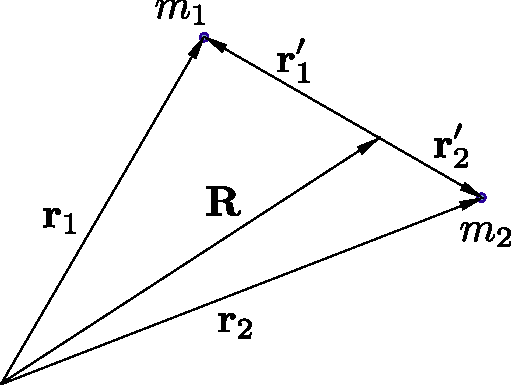
\includegraphics[width=0.4\textwidth]{images/fig_reduccion.pdf}	 
	\end{center}
	\caption{Sistema coordenado para la reducción del problema de dos cuperpos al de uno equivalente.}
\end{figure} 

Luego, como la energía se conserva (el $V_{cm}=cte.$) podemos escribir
\[
	E = \frac{1}{2} m_1 \dot{\vb{r}}_1^2 + \frac{1}{2} m_2 \dot{\vb{r}}_2^2 + V(r)
\]
\[
	E = \frac{1}{2} m_1 ( \dot{\vb{R}} + \dot{\vb{r}}_1' )^2 + \frac{1}{2} m_2 ( \dot{\vb{R}} + \dot{\vb{r}}_2' )^2 + V(r)
\]
\[
	E = \frac{1}{2} m_1 ( {\vb{V}} )^2 +  \frac{1}{2} m_1 ( \dot{\vb{r}}_1' )^2 + 
		\frac{1}{2} m_2 ( {\vb{V}})^2 + \frac{1}{2} m_2 (\dot{\vb{r}}_2' )^2 + V(r)
\]
\[
	E = \frac{1}{2} M {\vb{V}}^2 + \frac{1}{2} \frac{m_2^2}{m_1} \dot{\vb{r}}_2'^2 + \frac{1}{2} m_2 \dot{\vb{r}}_2'^2 + V(r)
\]
\[
	E = \frac{1}{2} M {\vb{V}}^2 + \frac{1}{2} \frac{m_2 m_1}{M} \dot{\vb{r}}^2 + V(r)
\]
y el 
\[
	e = \frac{1}{2} \mu \dot{\vb{r}}^2 + V(r)
\]
donde este último $\vb{r}$ es un vector distancia relativa. Es un problema equivalente para la partícula
centro de masas.
\[
	e = \frac{1}{2} \mu ( \dot{\vb{r}}^2 + r^2\dot{\phi}^2 ) + V(r)
\]

Diremos que la {\it distancia relativa} describe una elipse. Las trayectoria reales en el espacio físico
son dos elipses confocales. Por supuesto dejan de cumplirse las leyes de Kepler en este caso.

% =================================================================================================
\section{Dispersión}
% =================================================================================================

Consideramos la dispersión de un haz de partículas de cierta energía cinética por un centro dispersor,
ver ilustración.

\[
	d\sigma = \frac{dN}{n}
\]
donde $dN$ es el número de partículas dispersadas entre $\chi$ y $\chi + d\chi$ y $n$ es el número de
partículas emitidas por tiempo y por área. De esta forma $d\sigma$ tiene unidades de área.

Consideramos $d$ centro dispersor con simetría esférica (cilíndrica basta).
Usamos como suposiciones que todo lo que emerge entre $\rho + d\rho$ - $\rho$  es dispersado entre
$\chi + d\chi$ - $\chi$, y que se conservan tanto $E$ como \vb{L}.

El anillo se dispersa en un sector esférico. Entonces podemos establecer las siguientes conclusiones
para el anillo entre $\rho + d\rho$ - $\rho$, a saber
\[
	A =  \pi ( (\rho + d\rho)^2 - \rho^2 ) \qquad \longrightarrow A \approx 2 \pi \rho \: d\rho,
\]
entonces
\[
	d\sigma = \frac{  2 \pi \rho \: d\rho I}{I}
\]
donde $\rho$ es el parámetro de impacto y $I$ el número de partículas por unidad de tiempo y área.
Finalmente
\[
	d\sigma =  2 \pi \rho(\chi) \left| \dtot{\rho}{\chi} \right| d\chi
\]

Como se conservan la energía y el momento angular
\[
	E = \frac{1}{2} m V_\infty^2 \qquad L = m \rho V_\infty^2 
\]

En general se desconoce $V(r)$.

Se puede calcular el ángulo $\varphi_0$ de acuerdo a 
\[
	\chi = \pi - 2\varphi_0,
\]
donde
\[
	\varphi_0 = \int_{r_m}^{\infty} \frac{L/mr^2}{\sqrt{\frac{2}{m}(E - V_{eff})}} dr
\]
\[
	\chi = \pi - 2 \varphi_0 (\rho)
\]
e invertimos desde la última ecuación.

Veamos el caso de una esfera maciza. En general los cuerpos duros equivalen a un potencial del tipo
\[
	V = \begin{cases}
	     \infty \qquad \textrm{cuerpo}\\
	     \;0 \qquad \; \textrm{fuera} \\
	    \end{cases}
\]
\[
	\chi = \pi - 2\varphi_0
\]
\[
	\sin(\varphi_0) = \frac{\rho}{a} \qquad d\rho = -a \frac{1}{2}\cos \left(\frac{\pi-\chi}{2}\right)
\]
y entonces 
\[
	d\sigma = 2\pi a^2 \sin\left(\frac{\pi-\chi}{2}\right) \frac{1}{2}\cos\left(\frac{\pi-\chi}{2}\right) d\chi
\]
\[
	d\sigma = \frac{\pi}{2} a^2 \sin( \pi-\chi) d\chi = \frac{\pi}{2} a^2 \sin( \chi) d\chi
\]
y como hay que integrar $\chi$ de 0 a $\pi$
\[
	\int_0^\pi \frac{\pi}{2} a^2 \sin( \chi) d\chi = \pi a^2
\]
\[
	\sigma = \pi a^2
\]
En el caso de los cuerpos duros la sección eficaz es la sombra de los mismos.
\notamargen{Sobre el ángulo sólido
\[
\Omega = \textrm{Area}/r^2
\]
\[
d\Omega = 2 \pi \sin( \chi ) d\chi 
\]
\[
\Omega = 4 \pi 
\]
para la esfera.
}


% =================================================================================================
\section{Dispersión por dos cuerpos}
% =================================================================================================

Consideramos el caso de un cuerpo que se fracciona en dos (creo?)

Desde el centro de masa
\[
	\vb{P}_1 + \vb{P}_2 = 0
\]
\[
	m_1 \vb{v}_1 + m_2 \vb{v}_2 = 0
\]
definimos una velocidad relativa
\[
	\vb{v} \equiv \vb{v}_2  - \vb{v}_1 = \vb{v}_2 \left( \frac{ m_1 + m_2 }{ m_1 }\right) .
\]

Con respecto a la energía,
\[
	\frac{1}{2} M \vb{V}_{cm}^2 + e_{int} = \frac{1}{2} m_1 \vb{v}_1^2 + \frac{1}{2} m_2 \vb{v}_2^2
						+ e_{int 1 } + e_{int 2} + \frac{1}{2} M \vb{V}_{cm}^2
\]
\[
	\frac{1}{2} m_1 \vb{v}_1^2 + \frac{1}{2} m_2 \vb{v}_2^2 = e_{int} - e_{int 1 } - e_{int 2} = \Delta e
\]
y pasando todo en términos de la velocidad relativa
\[
	 \frac{1}{2} \frac{m1 m2}{ m_1 + m_2 } v = \Delta e
\]
entonces 
\[
	v = \sqrt{\frac{ 2 \Delta e}{ \mu } }.
\]

El problema es evidentemente plano.
\[
	\vb{V}_1^L =  \vb{V}_{cm} + \vb{V}_1' \qquad \longrightarrow \quad ( \vb{V}_1^L - \vb{V}_{cm} ) = \vb{V}_1'
\]
\[
	{V_1^L}^2 - V_{cm} - 2 {\vb{V}_1^L}^2 \vb{V}_{cm} = V_1^2
\]
\[
	{V_{1x}^L}^2 + {V_{1y}^L}^2 - V_{cm} - 2 {V_{1x}^L}^2 V_{cm} = V_1^2
\]
\[
	( V_{1x}^L  - V_{cm} )^2 + {V_{1y}^L}^2 = V_1^2
\]
que es una circunferencia.
\[
	\tan(\theta) = \frac{V_1 \sin(\chi) }{ V_{cm} + V_1 \cos(\chi) }
\]

Esto tiene dos raíces $\chi_{1,2}$ si $ V_{cm} > V_1$. 

Si $ V_{cm} > V_1$ hay una sola $V$ de las partículas.

Si $ V_{cm} < V_1$ hay partículas emitidas hacia atrás vistas desde L.

Si pensamos en una distribución isótropa de partículas, desde el centro de masa
\[
	e = \frac{1}{2} m_1 V_{1}^2
\]
\[
	V_L^2 = V_1^2 + V_{cm}^2 - 2 V_1 V_{cm} \cos( \pi -\chi )
\]
a iguales $V_1,V_{cm}$ se tienen variables $V_L, \chi$, entonces
\[
	dV_L^2 = - 2 V_1 V_{cm} \sin(\chi) d\chi
\]
\[
	\frac{dV_L^2}{2 V_1 V_{cm}} = \sin( \chi) d\chi 
\]
\[
	d\sigma = 2 \pi \rho |\dtot{\rho}{\chi}| d\chi 
\]
\[
	d\Omega = 2 \pi \sin( \chi ) d\chi 
\]
\[
	\frac{d\Omega}{4\pi} = \frac{1}{2} \sin( \chi ) d\chi 
\]
\[
	\frac{d\Omega}{4\pi} =  \frac{d (V_L^2) }{4 V_1 V_{cm}} = \frac{1}{2} \frac{d ( 1/2 m_1 V_L^2) }{m_1 V_1 V_{cm}} 
\]

% =================================================================================================
\section{Scattering}
% =================================================================================================

Tenemos dos suposiciones básicas:
	\begin{itemize}
		\item Interacción elástica.
		\item Conservación de energía y de momento.
	\end{itemize}
	
Desde el centro de masa se tienen:
\[
	\vb{P} = \vb{P}_1 + \vb{P}_2 = 0	\qquad		\vb{r} \equiv \vb{r}_2 + \vb{r}_1
	\qquad		\vb{V} \equiv \vb{V}_2 - \vb{V}_1
\]
donde los últimos son las posiciones y velocidades relativas.
\[
	E = \frac{1}{2} M \vb{V}_{cm}^2 + \frac{1}{2} \mu \vb{V}^2 + V(r)
\]
\[
	m_1 \vb{V}_1 + m_2 \vb{V}_2 = 0 \qquad m_1 \vb{V}_1 = -\frac{m_2}{m_1} \vb{V}_2.
\]

En términos de las velocidades relativas
\[
	\vb{V}_2 = \frac{m_1}{m_1 + m_2} \vb{V} \qquad \vb{V}_1 = -\frac{m_2}{m_1 + m_2} \vb{V}
\]
Se puede escribir la energía cinética del siguiente modo
\[
	T = \frac{1}{2} m_1 \vb{V}_{1-in}^2 + \frac{1}{2} m_2 \vb{V}_{2-in}^2 =
	\frac{1}{2} M \vb{V}_{cm}^2 + \frac{1}{2} m_1 \vb{V}_{1-cm}^2 + \frac{1}{2} m_2 \vb{V}_{2-cm}^2 
\]
\[
	T - \frac{1}{2} M \vb{V}_{cm}^2 \equiv t = \frac{1}{2} \frac{m_1 m_2}{m_1 + m_2} \vb{V}^2 =
							\frac{1}{2} \mu \vb{V}^2
\]

\[
	\vb{V}_1^L = \vb{V}_{cm} - \frac{m_2}{M} \vb{V}	\qquad \vb{V}_2^L = \vb{V}_{cm} - \frac{m_1}{M} \vb{V}
\]

\[
	\vb{p}_1^L = m_1 \vb{V}_{cm} - \mu \vb{V} = m_1 \frac{\vb{P}}{M} - \mu \vb{V}
\]
\[
	\vb{p}_2^L = m_2 \vb{V}_{cm} + \mu \vb{V} = m_2 \frac{\vb{P}}{M} + \mu \vb{V}
\]

Donde 
\[
	\vb{V}_{cm} + \vb{V}_1 = \vb{V}_1^L
\]
\[
	\vb{p}_2^L = \frac{m_2}{M} \vb{P} + \mu \vb{V}\hat{n}		\qquad	 \vb{p}_1^L = \frac{m_1}{M} \vb{P} - \mu \vb{V}\hat{n}
\]
\[
	\frac{m_2}{M} \vb{P} + \frac{m_1}{M} \vb{P} = \vb{P} = \vb{p}_2^L + \vb{p}_1^L
\]
\[
	\tan(\theta_2) = \frac{P_1 \sin(\chi)}{ (m_2/M) P + P_1\cos(\chi)}
\]

% =================================================================================================
\section{Dispersión por potenciales infinitos}
% =================================================================================================

La idea es que sabiendo $\rho$ (parámetro de impacto) quiero saber qué ángulo $\chi$ se desvían las
partículas incidentes.

\[
	\phi_0 + \alpha = \frac{\pi}{2}		\qquad		2 \phi_0 + \alpha + \beta = \pi
	\qquad \phi_0 + \beta = \frac{\pi}{2}
\]
\[
	\alpha = \beta		\qquad 		2\alpha = 2\beta = \chi
\]
\[
	\dtot{\rho}{z} = \tan \left(\beta \right) = \tan\left(\frac{\chi}{2}\right)
\]
\[
	\tan\left(\frac{\chi}{2}\right) = \dtot{\rho}{z} = \frac{ d\rho/dz }{ dz/d\theta }
\]
con $\theta$ variable paramétrica. Donde $\rho = \rho(z)$ es la función que da la curva roja (el perfil
del cuerpo dispersor).








% =================================================================================================

\bibliographystyle{CBFT-apa-good}	% (uses file "apa-good.bst")
\bibliography{CBFT.Referencias} % La base de datos bibliográfica

\end{document}
